%
% thesis.tex
%

\newcommand{\project}{$<<$project$>>$}
\newcommand{\doctitle}{Crossing the Streams}
\newcommand{\docsubtitle}{Functional Parallel Programming for Graphics Processing Units}
\newcommand{\doccontentsline}{Functional Programming for GPUs}


\documentclass[11pt,a4paper,twoside]{book}

% Imports
% ------------------------------------------------------------------------------

% \usepackage{pdf14}
% \usepackage[T1]{fontenc}
\usepackage{ifpdf}
\ifpdf
\RequirePackage{hyperref}
\hypersetup{%
    pdftitle={\doctitle},
    pdfsubject={\docsubtitle},
    pdfauthor={Trevor L. McDonell},
    colorlinks=false
}
\pdfcompresslevel=9
\fi

\usepackage{a4wide}
\usepackage{amsmath}
\usepackage{amssymb}
\usepackage{array}
\usepackage{booktabs}
\usepackage{calc}
\usepackage{caption}
\usepackage[usenames,dvipsnames]{xcolor}
\usepackage{doi}
\usepackage{epigraph}
\usepackage{fancyhdr}
% \usepackage{tipa}
\usepackage{fontspec}
\usepackage{graphicx}
\usepackage[all]{hypcap}
\usepackage{ifdraft}
\usepackage{ifthen}
% \usepackage{lastpage}
\usepackage[final]{listings}
% \usepackage{longtable}
\usepackage{makeidx}
\usepackage{marginnote}
\usepackage{mathtools}
\usepackage{mathrsfs}
\usepackage{mflogo}
\usepackage[numbers,sort&compress,nonamebreak]{natbib}
% \usepackage{pdfsync}
\usepackage{rotating}
\usepackage{setspace}
% \usepackage{showidx}
\usepackage[color]{showkeys}
\usepackage{subcaption}
\usepackage{titlesec}
\usepackage[width={autoauto}]{thumbs}
\usepackage{tabu}
\usepackage{textcomp}
\usepackage{tikz}
\usepackage{upquote}
\usepackage{xfrac}
\usepackage[multiple]{footmisc}

\onehalfspacing
%\doublespacing


% Draw numbers in circles
% ------------------------------------------------------------------------------

\newcommand*\circled[1]{\tikz[baseline=(char.base)]{
  \node[shape=circle,draw,inner sep=2pt] (char) {#1};}}

% Use symbols instead of numbers for footnote marks
% ------------------------------------------------------------------------------

%\renewcommand{\thefootnote}{$\fnsymbol{footnote}$}


% Bibliography
% ------------------------------------------------------------------------------

%\bibliographystyle{apsrev}             % citation order style
%\bibliographystyle{apsrmp}             % author/year style
\bibliographystyle{abbrvnat}
\providecommand{\bibfont}{\small}


% Figures and captions
% ------------------------------------------------------------------------------

% \message{The par indent is \the\parindent} ==> 17pt
\DeclareCaptionFormat{captionWithLine}{%
    \hspace{-8.5pt}\rule{\textwidth}{0.4pt}\\#1#2#3}
\captionsetup{margin=8.5pt,font=small,labelfont=bf}
% \captionsetup[subfloat]{margin=0pt,labelfont=default}

% Reduced bias to floats on their own page
%
% \renewcommand{\topfraction}{0.85}
% \renewcommand{\textfraction}{0.1}
% \renewcommand{\floatpagefraction}{0.75}


% Fancy header style
% ------------------------------------------------------------------------------

\newcommand{\sectionname}{Section}
\pagestyle{fancy}
\fancyhf{}
\renewcommand{\headrulewidth}{0pt}
\renewcommand{\chaptermark}[1]{\thispagestyle{empty}\markboth{#1}{}}
\renewcommand{\sectionmark}[1]{\markright{#1}}
\fancypagestyle{plain}{\fancyhf{}}
\fancyhead[EL]{\small\textsc{\thepage\hspace{2\medskipamount} \leftmark}}
%\fancyhead[ER]{\small\textsc{\chaptername\ \thechapter}}
%\fancyhead[OL]{\small\textsc{\sectionname\ \thesection}}
\fancyhead[OR]{\small\textsc{\rightmark\hspace{2\medskipamount} \thepage}}

\newcommand{\doccolor}{Bittersweet}
\newcommand{\docminorcolor}{Gray}


% Extra depth in numbered sections
% ------------------------------------------------------------------------------

%\setcounter{secnumdepth}{3}
%\setcounter{tocdepth}{3}
%\setcounter{lofdepth}{2}


% Citations
% ------------------------------------------------------------------------------

\let\Cite\cite
\renewcommand{\cite}{\nolinebreak\Cite}


% Keys and margin notes
% ------------------------------------------------------------------------------

% Showkeys
% texmf-dist/tex/latex/graphics/dvipsnam.def
%
% \definecolor{refkey}{cmyk}{0.0,0.89,0.94,0.28}        % BrickRed
% \definecolor{labelkey}{cmyk}{0.0,0.89,0.94,0.28}

% notes, margin notes, etc. delete for final mode
%
%\let\oldmarginnote\marginnote
%\providecommand{\marginnote}{\oldmarginnote }
\renewcommand*{\marginfont}{\color{BrickRed}\ttfamily\scriptsize}

\newcommand{\derp}{\textcolor{BrickRed}{derp}}
\newcommand{\note}[1]{\textcolor{BrickRed}{#1}}


% Code listings
% ------------------------------------------------------------------------------

% Fix spacing between chapter groups in the list of listings
%
% Unfortunately this _always_ adds the space, so the first entry is lower than
% it should be. We hack around this by adding some negative space to begin with.
%
\let\Chapter\chapter
\def\chapter{\addtocontents{lol}{\protect\addvspace{10pt}}\Chapter}
\addtocontents{lol}{\protect\vspace*{-20pt}}

\newfontfamily\sourcecodepro{Source Code Pro}
\newfontfamily\sourcecodeprobold{Source Code Pro Medium}
\newfontfamily\sourcecodeprolight{Source Code Pro Light}


% Define the language styles we will use
%
\lstset{%
    frame=none,
    rulecolor={\color[gray]{0.7}},
    numbers=none,
    basicstyle=\scriptsize\sourcecodepro,
    numberstyle=\color{Gray}\tiny\it,
    commentstyle=\color{MidnightBlue}\it,
    stringstyle=\color{Maroon},
    keywordstyle=[1],
    keywordstyle=[2]\color{ForestGreen},
    keywordstyle=[3]\color{Bittersweet},
    keywordstyle=[4]\color{RoyalPurple},
    captionpos=b,
    aboveskip=2\medskipamount,
    xleftmargin=0.5\parindent,
    xrightmargin=0.5\parindent,
    flexiblecolumns=false,
%   basewidth={0.5em,0.45em},           % default {0.6,0.45}
    escapechar={\%},
    texcl=true                          % tex comment lines
}

\lstloadlanguages{Haskell}

\lstdefinestyle{haskell}{%
    language=Haskell,
    upquote=true,
    deletekeywords={case,class,data,default,deriving,do,in,instance,let,of,type,where},
    morekeywords={[2]class,data,default,deriving,family,instance,type,where},
    morekeywords={[3]in,let,case,of,do},
    literate=
        {\\}{{$\lambda$}}1
        {\\\\}{{\char`\\\char`\\}}1
        {>->}{>->}3
        {>>=}{>>=}3
        {->}{{$\rightarrow$}}2
        {>=}{{$\geq$}}2
        {<-}{{$\leftarrow$}}2
        {<=}{{$\leq$}}2
        {=>}{{$\Rightarrow$}}2
        {|}{{$\mid$}}1
        {forall}{{$\forall$}}1
        {exists}{{$\exists$}}1
        {...}{{$\cdots$}}3
%       {`}{{\`{}}}1
%       {\ .}{{$\circ$}}2
%       {\ .\ }{{$\circ$}}2
}

\lstdefinestyle{cuda}{%
    language=CUDA,
    keywordstyle=[1]\color{ForestGreen},
    keywordstyle=[2]\color{Bittersweet},
    keywordstyle=[3]\color{BrickRed},
    keywordstyle=[4]\color{RoyalPurple},
    keywordstyle=[5]\color{Cyan},
    escapeinside={(@*}{*@)}
}

\lstdefinestyle{ptx}{%
    language=CUDA,
    mathescape=false,
    escapeinside={(@*}{*@)}
}

\lstdefinestyle{inline}{%
    style=haskell,
    basicstyle=\ttfamily,
    keywordstyle=[1],
    keywordstyle=[2],
    keywordstyle=[3],
    keywordstyle=[4],
    literate=
        {\\}{{$\lambda$}}1
        {\\\\}{{\char`\\\char`\\}}1
        {>->}{>->}3
        {>>=}{>>=}3
        {->}{{$\rightarrow$\space}}3    % include forced space
        {>=}{{$\geq$}}2
        {<-}{{$\leftarrow$}}2
        {<=}{{$\leq$}}2
        {=>}{{$\Rightarrow$}}2
        {|}{{$\mid$}}1
        {forall}{{$\forall$}}1
        {exists}{{$\exists$}}1
        {...}{{$\cdots$}}3
}

\lstdefinestyle{haskell_float}{%
    style=haskell,
%    frame=single,
%    numbers=left,
    float
}

\lstdefinestyle{cuda_float}{%
    style=cuda,
%    frame=single,
%    numbers=left,
    float
}


% Shorthand for inline code fragments
%
\newcommand{\code}[1]{\lstinline[style=inline];#1;}
\newcommand{\footcode}[1]{\lstinline[style=inline];#1;}

\newcommand{\makeatcode}{\lstMakeShortInline[style=inline]@}
\newcommand{\makeatchar}{\lstDeleteShortInline@}

\makeatcode
\newcommand{\app}{\ensuremath{\mathbin{\texttt{\char"40}}}}


% Chapter page style
% ------------------------------------------------------------------------------

% Epigraphs
%
\renewcommand{\textflush}{flushright}
\setlength{\epigraphwidth}{0.85\textwidth}
\setlength{\epigraphrule}{0pt}
\setlength{\afterepigraphskip}{1.5\baselineskip}


% Titlesec
%
\titleformat{\chapter}[display]%
    {\bfseries\Large}%
    {\vspace{-4ex}\filleft\Huge\thechapter}%
    {4pt}%
    {\filleft\titlerule[0.8pt]\vspace{1pt}\titlerule\vspace{2ex}}%
    [\vspace{2ex}{\titlerule[0.8pt]}\vspace{1pt}\titlerule]


% Index
% ------------------------------------------------------------------------------

\makeindex
\providecommand{\indexe}[1]{\index{#1}\emph{#1}}
\providecommand{\indext}[1]{\index{#1}#1}



\begin{document}

% FRONT MATTER
% ~~~~~~~~~~~~

\frontmatter
%
% title.tex
%

\phantomsection
\addcontentsline{toc}{chapter}{\doccontentsline}

\newlength{\centeroffset}
\setlength{\centeroffset}{-0.5\oddsidemargin}
\addtolength{\centeroffset}{0.5\evensidemargin}
\thispagestyle{empty}
\vspace*{\stretch{1}}
\noindent\hspace*{\centeroffset}\makebox[0pt][l]{
\begin{minipage}{\textwidth}
    \centering
    \hrule height 0.8pt
    \nobreak
    \vspace{1pt}
    \hrule
    \vspace{4ex}
    {\LARGE\bfseries \doctitle\\}
    \vspace{1ex}
    {\large\bfseries \docsubtitle}
    \vspace{4ex}
    \hrule height 0.8pt
    \nobreak
    \vspace{1pt}
    \hrule
\end{minipage}}

\vspace{4ex}
\noindent\hspace*{\centeroffset}\makebox[0pt][l]{
\begin{minipage}{\textwidth}
    \centering
    \textsc{\Large Trevor~L.~McDonell}\\[1.5ex]

    \textsc{School of Computer Science and Engineering}\\
    \textsc{University of New South Wales}

%    \textit{200220499}
%    \textcolor{White}{\textit{200220499}}
\end{minipage}}

\vspace{4ex}
\noindent\hspace*{\centeroffset}\makebox[0pt][l]{
\begin{minipage}{\textwidth}
    \centering
    \ifoptionfinal{\textcolor{White}{\today}}{\today}
\end{minipage}}

\vspace{6ex}
\noindent\hspace*{\centeroffset}\makebox[0pt][l]{
\begin{minipage}{\textwidth}
    \centering
    \hspace{0.5cm}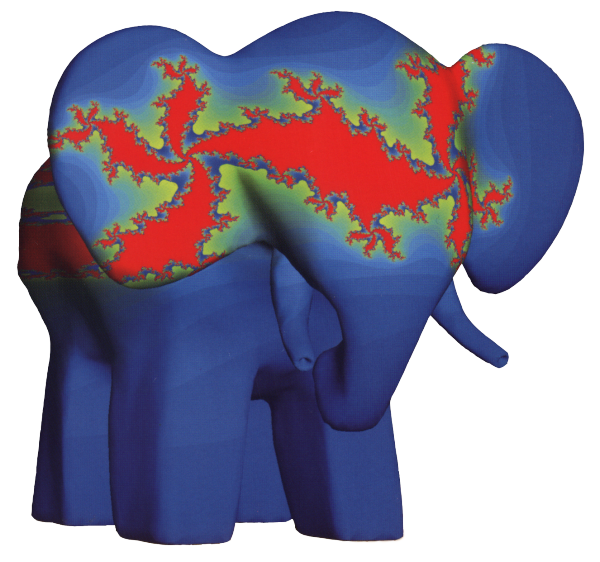
\includegraphics{images/sec-0/julia-elephant-s}
    \vspace*{1.87333708001in}	% height of julia-elephant-s

%    \hspace{0.5cm}
\includegraphics[height=1.87in]{images/misc/placeholder}
%    \vspace*{1.87in}
\end{minipage}}

\vspace{\stretch{2}}


%
% sec-i-disclaimer.tex
%

\pagebreak
\vspace*{\stretch{1}}
\noindent\makebox[0pt][l]{\begin{minipage}{\textwidth}
\flushleft
\begin{small}
%    Cover art: Rost, Randi~J., 1960--\\
%    OpenGL Shading Language / Randi J. Rost; with contributions from 
%    John M.~Kessenich \ldots\ [et al.]. --- 2nd ed.
%    (ISBN 0-321-33489-2)
%
%    \vspace{4ex}
%
%    \emph{\project} copyright \copyright\ 2009, Trevor L. McDonell\\
%    Original Author: Trevor L. McDonell (trevor.mcdonell@gmail.com)

    Copyright \copyright\ 2009--2012, Trevor L.\ McDonell
\end{small}
\end{minipage}}

%
% sec-ii-declaration.tex
%

\pagebreak
\vspace*{1in}
\noindent\makebox[0pt][l]{\begin{minipage}{\textwidth}
    \centering
    This thesis is submitted in partial fulfilment\\
    of the requirements for the degree of\\[3ex]

    \textsc{\ldots}\\[1.5ex]

%    \textsc{\large Bachelor of Engineering (Mechatronics (Space))}\\[1.5ex]
%    \textsc{\large Bachelor of Engineering (Mechatronics / Space Engineering)}\\[1.5ex]
%
%    \emph{and}\\[1.5ex]
%
%    \textsc{\large Bachelor of Science (Advanced)}\\[3ex]
%
%    School of Aerospace, Mechanical\\
%    and Mechatronic Engineering\\[1.5ex]
%    University of Sydney\\
%    Australia
\end{minipage}}


\cleardoublepage
\vspace*{1in}
\noindent\makebox[0pt][l]{\begin{minipage}{\textwidth}
    \centering
    I hereby declare that this submission contains my own work,\\
    and includes no material which to a substantial extent has been 
    performed by others,\\
    except where otherwise acknowledged.
\end{minipage}}

\vspace{1in}
\noindent\makebox[0pt][l]{\begin{minipage}{\textwidth}
    \centering
    \hfill{} \textsc{trevor l. mcdonell} \hfill{} \textsc{date} \hfill{}
\end{minipage}}



% Contents pages (only in book mode)
%
\cleardoublepage
\phantomsection
\addcontentsline{toc}{chapter}{Contents}
\tableofcontents\markboth{Contents}{Contents}

\cleardoublepage
\phantomsection
\renewcommand{\listfigurename}{Figures}
\addcontentsline{toc}{chapter}{\listfigurename}
\listoffigures\markboth{\listfigurename}{\listfigurename}

\cleardoublepage
\phantomsection
\addcontentsline{toc}{chapter}{\lstlistlistingname}
\lstlistoflistings\markboth{\lstlistlistingname}{\lstlistlistingname}
\addtocontents{lol}{\vspace{10pt}}


\chapter{Abstract}
\markboth{Abstract}{}

Computers are no longer getting faster. Instead, including multiple cores on a
single chip has become the dominant mechanism for scaling processor performance,
and the exponential growth in the number of cores on a single processor is
expected to lead in a short time to mainstream computers containing hundreds of
devices. Unfortunately, programming parallel computers is known to be an
extremely challenging task, even for expert computer programmers.

In order to achieve improved single-application performance on such processors,
an appropriate programming model is needed which can expose parallelism and
address scalability. Commodity graphics processing units, which have evolved
into flexible general-purpose parallel architectures, can provide some insight
into many of the challengers developers will face; finding parallelism within
our applications to satiate available hardware, and rationalising the
interactions of large numbers of concurrent threads.

This thesis presents the design, implementation, and evaluation of a new
domain--specific language embedded within Haskell for flat data-parallel array
computations executed on graphics processing units. The design concentrates on
providing a high--level abstraction that composes computations that run
efficiently according to the strengths and weaknesses of the underlying
hardware, without forcing the programmer to recast their algorithm to fit within
the architecture.

The final design \ldots\ and benchmarking shows that the goals of the design were
\ldots


%          File: sec-iv-acknowledgements.tex
%       Created: Sat 07 Oct 2006 03:11:37 PM EST
% Last Modified: Mon 23 Oct 2006 12:03:27 PM EST

\chapter{Acknowledgements}
\markboth{Acknowledgements}{}



% MAIN MATTER
% ~~~~~~~~~~~

\mainmatter
\fancyhead[ER]{\small\textsc{\chaptername\ \thechapter}}
\fancyhead[OL]{\small\textsc{\sectionname\ \thesection}}

% Use symbols instead of numbers for footnote marks
%
\renewcommand{\thefootnote}{$\fnsymbol{footnote}$}

% Add chapter thumbs for the main matter section only. At the beginning of the
% back matter we stop displaying thumbs and revert to \oldchapter
%
\let\oldchapter\chapter
\renewcommand{\chapter}[1]{\oldchapter{#1}\addthumb{#1}{}{white}{black}}

% include three years of work...
%

\chapter{Introduction}
\epigraph{First things first, but not necessarily in that order.}
{\textsc{---the doctor}}

%\epigraph{Come then, and let us pass a leisure hour in 
%storytelling,\\and our story shall be the education of our heroes.}%
%{\textsc{---plato}\\\textit{Republic}, \textsc{book ii}}

\textcolor{red}{This needs to be redone}

Over the last ten years, an interesting trend in computing has emerged. General
purpose CPUs, such as those provided by Intel, IBM and AMD, have increased
performance substantially, but with nowhere near the increases seen in the late
1980's and early 1990's. To a large extent, single threaded performance
increases have tapered off due to the low level of inter-process communication
in general purpose workloads, and the physical limitations of power dissipation
for integrated circuits. The additional millions and billions of transistors
afforded by Moore's Rule\footnote{Moore's actual prediction in 1965 referred
only to the number of devices that could be fabricated on a single die, and that
this quantity would increase by fifty percent each year \cite{Moore:1965wc}.}
are simply not very productive in increasing the performance of single--threaded
code.

At the same time, the commodity \indexe{graphics processing unit} (GPU) has been
able to use this ever increasing transistor budget effectively, geometrically
increasing rendering performance, since rasterisation is an inherently parallel
operation. Historically fixed function pipelines, modern graphics architectures
have evolved to become increasingly flexible as well as powerful, consisting of
an expressive set of general purpose computation resources, with some fixed
function units on the side.

Parallel programming models fall into two broad categories. Task parallelism
emphasises a distributed model for independent processes, whereas data
parallelism specifies a single computation which is applied simultaneously
across a large number of data elements. While task parallelism typically does not
scale well with the size of the problem, data parallelism provides one of the
most promising approaches to making efficient use of parallel hardware.

Despite their attractiveness for computationally intensive operations, accessing
this performance has remained elusive for all but a few applications. The
arithmetic power of the GPU is a result of a highly specialised and constrained
architecture, resulting in programs which rely heavily on the CPU to handle
difficult parts of control and data flow. However, the CPU--GPU link is
relatively slow, engendering high communication latencies which radically impair
performance. To be practicable, the GPU programming model must efficiently
support messy boundary conditions, irregular data and control flow patterns, and
provide an elegant mapping from the application to the underling architecture,
without forcing the programmer to recast their algorithm. Support for nested
data parallelism \cite{Blelloch:1994vc,Blelloch:1996jx} (NDP) would provide a
first step towards a viable GPU programming model, unshackling vast
computational resources from the small application niche for which they were
originally designed.


%
% Background / Literature Review
%
% The literature review is an organisational pattern that combines both summary
% and synthesis. It may give a new interpretation of old material, combine old
% and new interpretations, or trace the intellectual progression of a field. It
% should be organised around ideas, not expand each source individually.
%
% - What themes and issues connect the sources together?
% - What solutions are present, which aspects are missing?
% - What is the trend in the field?
%

\chapter{Background}
\epigraph{Why waste time learning, when ignorance is instantaneous?}
{\textsc{---calvin and hobbes}}
\label{ch:background}

%
% Progression:
%  1. Technology trends, move towards increasing parallelism
%  2. Parallel computing, introduce NDP and speedup/code -> inf promise
%  3. GPGPU. Short history. Problems, need for reuse, abstraction from HW
%  4. Develop a need/motivation to combine (2) and (3)
%
% Organisation:
%  1. Introduction: quick idea of the topic, central theme
%  2. Body: sources thematically
%  3. Conclusion and recommendations
%
%  + Models and Languages for Parallel Computing
%    + Challenges to Parallel Computing
%    + Approaches to Parallel Computing
%    + Evaluating Parallel Programs
%
%  + Parallel Programming for Graphics Processing Units
%  + CUDA
%    + Hardware Model
%    + Programming Model
%    + Execution Control
%    + Memory Model
%
%  + Motivation
%

\begin{itemize}
    \item Functional programming 101
        \begin{itemize}
            \item Haskell 101?
            \item bulk programming; function composition
            \item denotional semantics?
        \end{itemize}

    \item Parallel programming 101 (steal from literature review)
        \begin{itemize}
            \item parallel vs. concurrent
            \item data parallelism
                \begin{itemize}
                    \item example parallel programming operators (fold, scan)
                    \item parallel interpretation of ostensibly serial
                        operations
                \end{itemize}
            \item evaluating parallel programs
                \begin{itemize}
                    \item work and depth complexity
                    \item parallel speedup
                    \item wall clock time!
                \end{itemize}
        \end{itemize}

    \item CUDA programming 101
        \begin{itemize}
            \item GPGPU programming
                \begin{itemize}
                    \item why bother?
                    \item performance vs. development time
                \end{itemize}
            \item programming model
                \begin{itemize}
                    \item SIMD architecture
                    \item kernels, thread blocks
                    \item memory \& coalescing
                \end{itemize}
        \end{itemize}

    \item Embedded languages
        \begin{itemize}
            \item advantages: using tools/features of host language
            \item deep vs. shallow. \url{http://skillsmatter.com/podcast/scala/making-edsls-fly}
            \item DSLs in Haskell
                \begin{itemize}
                    \item simple (untyped) DSL
                    \item GADTs to encode type safety / invariants
                    \item type-safe evaluator
                    \item itemize design requirements / goals of this language
                \end{itemize}
        \end{itemize}

\end{itemize}



Modern microprocessor technology is constructed from millions of interconnected
switching devices, called transistors. As process technology advances, these
transistors, and the interconnections between them, can be fabricated in a
smaller area. The challenge for microprocessor architects is to translate this
increase in resources into an increase in performance.

Unfortunately, computers are no longer getting faster. Instead, we are being
offered computers containing more and more CPUs, each of which is individually
not substantially faster than those of the previous generation. As the number of
processors increases, it will become increasingly important for programmers to
utilise these additional processing elements.

Processor designs are clearly evolving in one direction: towards massive
parallelism and many-core architectures. Unfortunately, the model of programming
used in mainstream languages was developed many years ago, when programs were
sequential and architectures were relatively simple. As hardware architectures
become larger and more complex, these traditional low-level approaches to
parallel programming become less and less tractable for real applications.

This section \ldots


\section{Parallel Programming}

Programming parallel computers is an extremely challenging task. This is true
even for expert computer programmers, let alone for scientists in other
disciplines whose computations are often what drive the acquisition of
high-performance machines. For many years, parallel computing has waned in and
out of favour, alternatively seen as the solution to all computational
limitations or a waste of time, given the rate at which processor and memory
speeds improve. These changing perceptions are the result of many factors,
including the programming environments available to users, the types of
supercomputing hardware on offer from vendors, and continual changes in the
focus of the academic community as to what are the ``hot'' problems of the time.

Nevertheless, the promise of parallel computing remains the same today as it was
at its inception. If users can buy sequential computers with gigabytes of
memory, imagine how much faster their programs could run if \emph{p} of these
machines were working cooperatively; imagine how much larger a problem could be
solved if the memories of these \emph{p} machines were used collectively.

The challenges to realising this potential faces two main difficulties; the
hardware, and the software. The former asks ``how do I build a parallel computer
that will allow these \emph{p} processors and memories to cooperate
efficiently?'' Then, given such a platform the latter asks ``how do I express my
computation such that it will utilise these \emph{p} processors and memories
effectively?''

In recent years there has been a growing awareness that while the parallel
computing community can build machines that are reasonably efficient and
affordable, the population of users that can effectively program these machines
comprises only a small fraction of those who can program traditional sequential
computers. Moreover, even the best parallel programmers can not do so without
significant effort. Parallel programming is still seen by many as an arcane
skill, a black art; best avoided if possible.

However, recent changes to the landscape of computing hardware will likely force
even mainstream application developers to abandon the ways of sequential
programming. In order to continually increase performance, compiler and
processor designers have struggled to to automatically exploit the implicit
parallelism present in serial programs. Using this technique, instructions can
be rescheduled in order to best exploit the multiple functional units available
in superscalar architectures. However, experience has shown that most serial
programs contain limited implicit parallelism \cite{Wall:1991}. While
techniques exist that can raise this limit somewhat, they come at the cost of
increased power to performance ratios and hardware complexity. Automatic
extraction of parallelism without explicit assistance from the programmer has
reached the point of diminishing returns. Including multiple cores on a single
chip has now become the dominant mechanism for scaling processor performance,
and there is renewed interest in parallel programming models, languages and
platforms.

At the same time, one must concede that programming a parallel machine is
inherently more difficult than sequential programming, as programmers must think
not only of correctness but concurrency and communication as well. It
undoubtedly complicates a programmer's life, but there is no silver bullet.
However, a good programming model should be able to unburden the programmer from
dealing with trivia, automating the more tedious aspects of mapping the
computation to the target hardware. Ideally, the programmer should focus on
%making major policy decisions and on
designing a correct and efficient algorithm.


\section{Haskell}
%
% Possible; Haskell compared to:
%   + static languages
%   + dynamic languages
%

\indexe{Haskell} is a general-purpose \emph{purely functional programming
language} with \emph{non-strict semantics} \index{non-strict semantics|see{lazy}}
and \emph{strong static typing}\index{typing!static}. In an imperative programming
language you get things done by giving the computer a sequence of actions to
perform and letting it execute them. While executing these statements the
computer is typically allowed to change some state: setting some variable
\texttt{ans} to $42$, doing some stuff, and then changing \texttt{ans} to
something else. In contrast, purely functional programming is not so much
concerned with telling the computer what to \emph{do} in so much as telling it
what stuff \emph{is}. The factorial of a number is the product of all the
numbers from one to that number; the sum of a list of numbers is the first
number plus the sum of the rest of the numbers; and so on. This is expressed in
the form of \emph{functions}, and programs can then be thought of as a sequence
of functions applying a series of transformations on data.

Haskell is a \indexe{pure} language; if you say some variable \texttt{ans} has
the value $42$, you can not later say that it has a different value. We assert
that pure functions like this do not have any \indexe{side effects}: the only
thing they can do is to perform some calculation on their inputs and return a
result. This might at first seem limiting, but has a rather nice consequence: if
a function is called twice with the same inputs, it will always return the same
result. This is known as \indexe{referential transparency} and not only allows
the compiler to reason about the behaviour of the program, but also allows the
user to deduce the \indexe{correctness} of a function and to build complex
functions by gluing together simpler functions.

Haskell is a \emph{statically typed}\index{typing!static} language; when you
compile your program the compiler knows which piece of code is a number, which
is a string, and so on. As such many possible errors are caught at compilation
time; the compiler will complain if you attempt to add a number to a string, for
example. Haskell uses a very good system of type inference based on
Hindley--Milner \textcolor{blue}{[citation needed]}, so that you don't have to
explicitly label each piece of code with a type.

Haskell is a \indexe{lazy} language; unless told otherwise it will not
explicitly evaluate functions or calculate values until a result is actually
required. Lazy evaluation might seem to have some spooky effects, but goes in
hand with the idea of referential transparency and profoundly affects how one
writes programs.

While Haskell encourages the pure, lazy style of functional program, this is
merely the default option. Haskell supports stateful functions, using distinct
types for functions with side effects orthogonal to the type of pure functions,
ensuring the two can not be conflated. While the focus of the language is
writing statically typed programs it is possible, although rare, to write
dynamically typed programs as well.


% \subsection{Syntax}
% basic crash course necessary?

% \subsection{Style}


\section{CUDA}


%
% sec-3-design.tex
%
% Embedded languages, stratified types, richly typed terms, representing
% programs. The Accelerate language.
%
% Accelerate CUDA backend. Code generation. Executing computations. Garbage
% collection. Caching.
%

\chapter{Design}
\epigraph{You see a wile, you thwart. Am I right?}%
{\textsc{---terry pratchett and neil gaiman}\\\textit{Good Omens}}

\begin{itemize}
    \item design of a stratified language (steal from DAMP)
        \begin{itemize}
            \item using the type system to exclude nesting
            \item richly typed terms; environments \& types
            \item types $\Rightarrow$ correctness??
            \item surface \& internal (core) languages
            \item representing different constructs (c.f. nesting?)
        \end{itemize}

    \item Related work, why it sucks
        \begin{itemize}
            \item open source: C/C++, Python, Haskell
            \item commercial: Matlab (Jacket), ArrayFire
        \end{itemize}

    \item Why another parallel programming language?
        \begin{itemize}
            \item expressiveness? (NDP \#fail \#sadface)
            \item ease of use?
        \end{itemize}

    \item Accelerate \textit{design}
        \begin{itemize}
            \item programming model
            \item algorithmic skeletons
            \item examples: operator expressiveness (application driven)
        \end{itemize}

\end{itemize}



%
% sec-4-implementation.tex
%

\chapter{Implementation}
\epigraph{The trouble with opportunity is that it always comes disguised 
as hard work.}%
{\textsc{---herbert v. prochnow}}



%
% sec-5-results.tex
%

\chapter{Results}
\epigraph{Dionysus [is] the Master of Illusions, who could make a vine 
grow out of a ship's plank, and in general enable his votaries to see 
the world as the world's not.}%
{\textsc{---e.\ r.\ dodds}\\\textit{The Greeks and the Irrational}}


%
% sec-6-conclusion.tex
%

\chapter{Conclusion}
\epigraph{The best way to predict the future is to implement it.}
{\textsc{---david heinemeier hansson}}



% BACK MATTER
% ~~~~~~~~~~~

\cleardoublepage
\
\backmatter
\stopthumb
\let\chapter\oldchapter
\fancyhead[ER]{}
\fancyhead[OL]{}

\cleardoublepage
\phantomsection
\addcontentsline{toc}{chapter}{Bibliography}
\bibliography{thesis}

\cleardoublepage
\phantomsection
\addcontentsline{toc}{chapter}{Index}
\printindex\markboth{Index}{Index}

\end{document}

